\documentclass[11pt,a4paper]{article}

% --------------------------------------------------
% Packages
% --------------------------------------------------
\usepackage[a4paper,margin=1in]{geometry}
\usepackage{amsmath,amssymb}
\usepackage{graphicx}
\usepackage{booktabs}
\usepackage{float}
\usepackage{siunitx}
\usepackage{hyperref}
\usepackage{xcolor}
\usepackage{caption}
\usepackage{subcaption}

\hypersetup{
    colorlinks=true,
    linkcolor=blue,
    urlcolor=blue,
    citecolor=blue
}

% --------------------------------------------------
% Document Information
% --------------------------------------------------
\title{
    \textbf{Stage 2: Frequency Analysis Using FFT} \\
    \large Engineering Signal Processing Lab
}

\author{
    Mohammad Umair Naeem
}

\date{\today}

\begin{document}

\maketitle

% --------------------------------------------------
\section{Project Premise}
% --------------------------------------------------

Stage 2 focuses on frequency-domain analysis of vibration signals using the Fast Fourier Transform (FFT). The objective is to transform time-domain vibration signals into frequency-domain representations and extract useful spectral information such as dominant frequencies, amplitudes, phase values, power spectral density, zero-padding effects, spectral leakage, windowing effects, and harmonic components.

The stage builds directly on Stage 1, where synthetic vibration signals were generated in the time domain. In this stage, those signals are analyzed to identify the frequency components embedded within them.

The computational work is implemented in Python using reusable functions and separate experiment scripts. The main implementation file is:

\begin{verbatim}
stage_02_fft_frequency_analysis/src/spectral_analysis.py
\end{verbatim}

The experiment scripts are:

\begin{verbatim}
01_amplitude_spectrum.py
02_phase_spectrum.py
03_power_spectral_density.py
04_zero_padding.py
05_harmonic_detection.py
06_spectral_leakage_windowing.py
\end{verbatim}

% --------------------------------------------------
\section{Engineering Relevance}
% --------------------------------------------------

Frequency analysis is fundamental in structural dynamics and structural health monitoring (SHM). Structural vibration data is usually measured in the time domain using accelerometers, displacement sensors, or velocity sensors. However, many important structural properties are easier to interpret in the frequency domain.

In SHM, frequency-domain analysis is useful for:

\begin{itemize}
    \item identifying dominant vibration frequencies,
    \item estimating possible natural frequencies,
    \item observing shifts in modal frequencies,
    \item detecting excitation frequencies,
    \item separating noise from meaningful vibration content,
    \item studying harmonic behavior,
    \item supporting modal identification and damage-sensitive feature extraction.
\end{itemize}

For example, if a structure loses stiffness due to damage, its natural frequency may decrease. Therefore, tracking frequency peaks over time can provide a useful indicator of structural change.

% --------------------------------------------------
\section{Theoretical Background}
% --------------------------------------------------

A vibration signal measured from a structure is commonly represented as a discrete time-domain signal:

\begin{equation}
    x[n], \qquad n = 0,1,2,\dots,N-1
\end{equation}

where \(x[n]\) is the sampled signal and \(N\) is the number of samples.

The sampling frequency is denoted by \(f_s\), and the sampling interval is:

\begin{equation}
    \Delta t = \frac{1}{f_s}
\end{equation}

The FFT converts the discrete time-domain signal into a discrete frequency-domain representation. The FFT does not directly return physical frequencies. Instead, it returns frequency bins. These bins are mapped to physical frequencies using the sampling frequency and the number of samples.

The frequency spacing is:

\begin{equation}
    \Delta f = \frac{f_s}{N}
\end{equation}

Equivalently, since the total duration is:

\begin{equation}
    T = \frac{N}{f_s}
\end{equation}

the frequency spacing can also be written as:

\begin{equation}
    \Delta f = \frac{1}{T}
\end{equation}

This means that longer measurement duration provides finer true frequency resolution.

% --------------------------------------------------
\section{Mathematical Formulation}
% --------------------------------------------------

\subsection{Discrete Fourier Transform}

The Discrete Fourier Transform (DFT) of a discrete signal \(x[n]\) is:

\begin{equation}
    X[k] =
    \sum_{n=0}^{N-1}
    x[n] e^{-j 2\pi kn/N}
\end{equation}

where:

\begin{itemize}
    \item \(x[n]\) is the time-domain signal,
    \item \(X[k]\) is the complex frequency-domain coefficient,
    \item \(N\) is the number of samples,
    \item \(k\) is the frequency bin index,
    \item \(j = \sqrt{-1}\).
\end{itemize}

The FFT is an efficient algorithm for computing the DFT. It gives the same mathematical result as the DFT but with much lower computational cost.

\subsection{Frequency Bins}

The frequency corresponding to bin \(k\) is:

\begin{equation}
    f_k = \frac{k f_s}{N}
\end{equation}

where \(f_k\) is the physical frequency in hertz.

For example, if:

\begin{equation}
    f_s = 100 \ \si{Hz}, \qquad N = 500
\end{equation}

then:

\begin{equation}
    \Delta f = \frac{100}{500} = 0.2 \ \si{Hz}
\end{equation}

Therefore, the FFT bins are located at:

\begin{equation}
    0,\ 0.2,\ 0.4,\ 0.6,\dots \ \si{Hz}
\end{equation}

\subsection{Single-Sided Amplitude Spectrum}

The FFT output \(X[k]\) is complex. The magnitude of each coefficient is:

\begin{equation}
    |X[k]| = \sqrt{\Re(X[k])^2 + \Im(X[k])^2}
\end{equation}

For a real-valued vibration signal, the FFT contains positive and negative frequency components. The negative-frequency part is the mirror image of the positive-frequency part. Therefore, only the positive-frequency side is usually retained.

The normalized single-sided amplitude spectrum is computed as:

\begin{equation}
    A[k] = \frac{|X[k]|}{N}
\end{equation}

For non-DC positive-frequency components, the amplitude is doubled:

\begin{equation}
    A_{\text{single}}[k] =
    \frac{2|X[k]|}{N}
\end{equation}

This correction is required because half of the spectral content was originally represented in the negative-frequency side.

The DC component at \(0\ \si{Hz}\) is not doubled. If the Nyquist frequency is present, it is also not doubled.

\subsection{Phase Spectrum}

The phase spectrum is obtained from the angle of the complex FFT coefficient:

\begin{equation}
    \phi[k] = \angle X[k]
\end{equation}

or equivalently:

\begin{equation}
    \phi[k] =
    \tan^{-1}
    \left(
        \frac{\Im(X[k])}{\Re(X[k])}
    \right)
\end{equation}

The phase gives the relative shift of each frequency component. In structural monitoring, phase becomes important when comparing vibration signals measured at different sensor locations.

\subsection{Power Spectral Density}

The Power Spectral Density (PSD) describes how signal power is distributed over frequency. While the amplitude spectrum is useful for clean deterministic signals, the PSD is more useful for noisy or random vibration data.

For a windowed signal segment \(x_m[n]w[n]\), the FFT is:

\begin{equation}
    X_m[k] =
    \sum_{n=0}^{L-1}
    x_m[n] w[n] e^{-j2\pi kn/L}
\end{equation}

where:

\begin{itemize}
    \item \(m\) is the segment index,
    \item \(L\) is the segment length,
    \item \(w[n]\) is the window function.
\end{itemize}

The window normalization factor is:

\begin{equation}
    U =
    \frac{1}{L}
    \sum_{n=0}^{L-1} w^2[n]
\end{equation}

The periodogram estimate for segment \(m\) is:

\begin{equation}
    P_m[k] =
    \frac{|X_m[k]|^2}{f_s L U}
\end{equation}

Welch's PSD estimate is obtained by averaging the periodograms from \(M\) overlapping segments:

\begin{equation}
    P_{\text{Welch}}[k] =
    \frac{1}{M}
    \sum_{m=1}^{M} P_m[k]
\end{equation}

This averaging reduces random fluctuations in the spectrum and produces a smoother PSD estimate.

\subsection{Zero-Padding}

Zero-padding means adding zeros to the end of a time-domain signal before computing the FFT. If the original signal has \(N\) samples and the padded FFT length is \(N_{\text{pad}}\), then:

\begin{equation}
    N_{\text{pad}} > N
\end{equation}

The padded frequency spacing becomes:

\begin{equation}
    \Delta f_{\text{pad}} =
    \frac{f_s}{N_{\text{pad}}}
\end{equation}

However, zero-padding does not increase the true physical frequency resolution. The true resolution is governed by the actual recorded duration:

\begin{equation}
    \Delta f_{\text{true}} =
    \frac{1}{T}
\end{equation}

Zero-padding only creates a denser frequency grid and produces a smoother-looking spectrum.

\subsection{Spectral Leakage}

Spectral leakage occurs when a signal does not contain an integer number of cycles within the observation window. In such cases, the signal frequency does not fall exactly on an FFT bin, and its energy spreads into neighboring bins.

If the FFT bin spacing is \(\Delta f\), and the signal frequency \(f\) is not equal to any bin frequency \(f_k\), then:

\begin{equation}
    f \neq k \Delta f
\end{equation}

This produces leakage around the true frequency.

\subsection{Hann Window}

A Hann window is commonly used to reduce spectral leakage. It is defined as:

\begin{equation}
    w[n] =
    \frac{1}{2}
    \left(
    1 - \cos
    \left(
    \frac{2\pi n}{N-1}
    \right)
    \right),
    \qquad 0 \leq n \leq N-1
\end{equation}

The window gradually reduces the signal amplitude at the beginning and end of the time record, reducing the artificial discontinuity created by finite-length sampling.

\subsection{Harmonic Detection}

Harmonics are frequencies that occur at integer multiples of a fundamental frequency:

\begin{equation}
    f_h = h f_0
\end{equation}

where:

\begin{itemize}
    \item \(f_0\) is the fundamental frequency,
    \item \(h = 1,2,3,\dots\) is the harmonic number,
    \item \(f_h\) is the harmonic frequency.
\end{itemize}

A detected peak frequency \(f_i\) is classified as harmonic if:

\begin{equation}
    \left|
    \frac{f_i}{f_0} - h
    \right|
    \leq \epsilon
\end{equation}

where \(\epsilon\) is the allowed tolerance.

% --------------------------------------------------
\section{Implementation Overview}
% --------------------------------------------------

The implementation is organized into reusable functions and experiment scripts.

The reusable module contains functions for:

\begin{itemize}
    \item computing the single-sided FFT amplitude spectrum,
    \item computing the phase spectrum,
    \item detecting frequency peaks,
    \item estimating PSD using Welch's method,
    \item detecting harmonic relationships,
    \item computing frequency resolution.
\end{itemize}

The general computational workflow is:

\begin{enumerate}
    \item Generate or import a time-domain vibration signal.
    \item Define sampling parameters \(f_s\), \(\Delta t\), \(N\), and duration.
    \item Compute FFT using NumPy.
    \item Convert FFT bins to physical frequency values.
    \item Retain the positive-frequency side.
    \item Scale the amplitude spectrum correctly.
    \item Detect dominant frequency peaks.
    \item Compute phase or PSD where required.
    \item Interpret results from a structural dynamics perspective.
\end{enumerate}

The implementation does not treat FFT as a black-box plotting command. Instead, it explicitly connects the mathematical quantities \(X[k]\), \(f_k\), \(A[k]\), \(\phi[k]\), and \(P_{\text{Welch}}[k]\) to the Python calculations.

% --------------------------------------------------
\section{Experiments}
% --------------------------------------------------

\subsection{Experiment 1: FFT Amplitude Spectrum}

\subsubsection{Premise}

A synthetic vibration signal is generated using two sinusoidal components. The objective is to verify that the FFT amplitude spectrum can recover the correct frequency and amplitude of each component.

\subsubsection{Signal Definition}

\begin{equation}
    x(t) =
    1.5 \sin(2\pi 5t)
    +
    0.8 \sin(2\pi 15t)
\end{equation}

\subsubsection{Parameters}

\begin{table}[H]
\centering
\caption{Parameters for FFT amplitude spectrum experiment}
\begin{tabular}{ll}
\toprule
Parameter & Value \\
\midrule
Sampling frequency, \(f_s\) & \(100\ \si{Hz}\) \\
Duration, \(T\) & \(5\ \si{s}\) \\
Number of samples, \(N\) & \(500\) \\
Frequency resolution, \(\Delta f\) & \(0.2\ \si{Hz}\) \\
Frequency component 1 & \(5\ \si{Hz}\) \\
Amplitude component 1 & \(1.5\) \\
Frequency component 2 & \(15\ \si{Hz}\) \\
Amplitude component 2 & \(0.8\) \\
\bottomrule
\end{tabular}
\end{table}

\subsubsection{Results}

The FFT amplitude spectrum is expected to show two dominant peaks.

\begin{table}[H]
\centering
\caption{Expected dominant frequency peaks}
\begin{tabular}{lll}
\toprule
Peak & Frequency & Amplitude \\
\midrule
1 & \(5\ \si{Hz}\) & \(1.5\) \\
2 & \(15\ \si{Hz}\) & \(0.8\) \\
\bottomrule
\end{tabular}
\end{table}

\subsubsection{Generated Figure}

\begin{figure}[H]
\centering
\begin{subfigure}{0.48\textwidth}
\centering
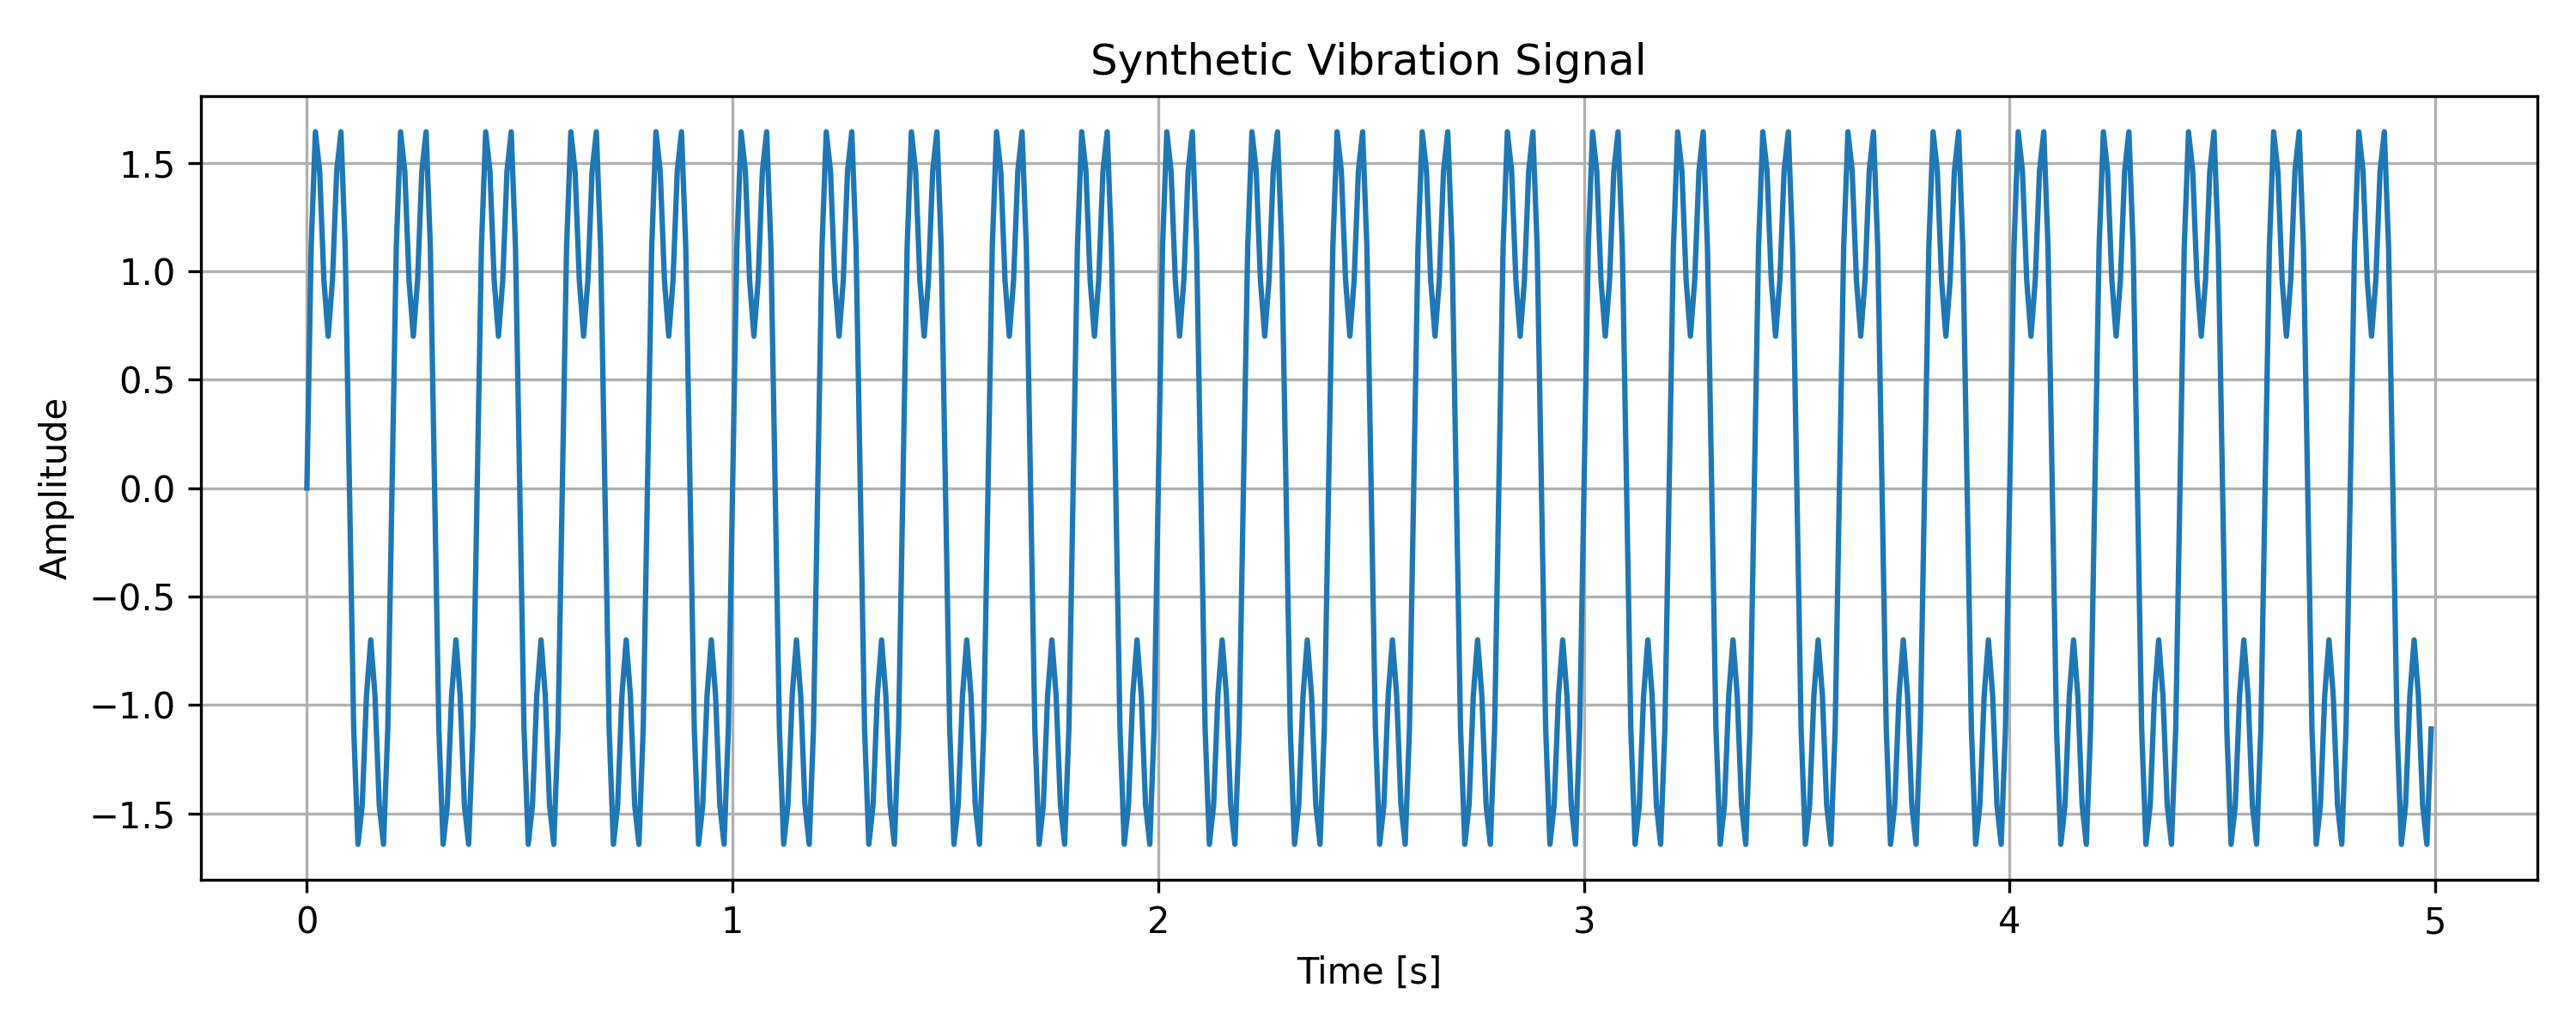
\includegraphics[width=\textwidth]{figures/exp01_time_signal.png}
\caption{Time-domain signal.}
\end{subfigure}
\hfill
\begin{subfigure}{0.48\textwidth}
\centering
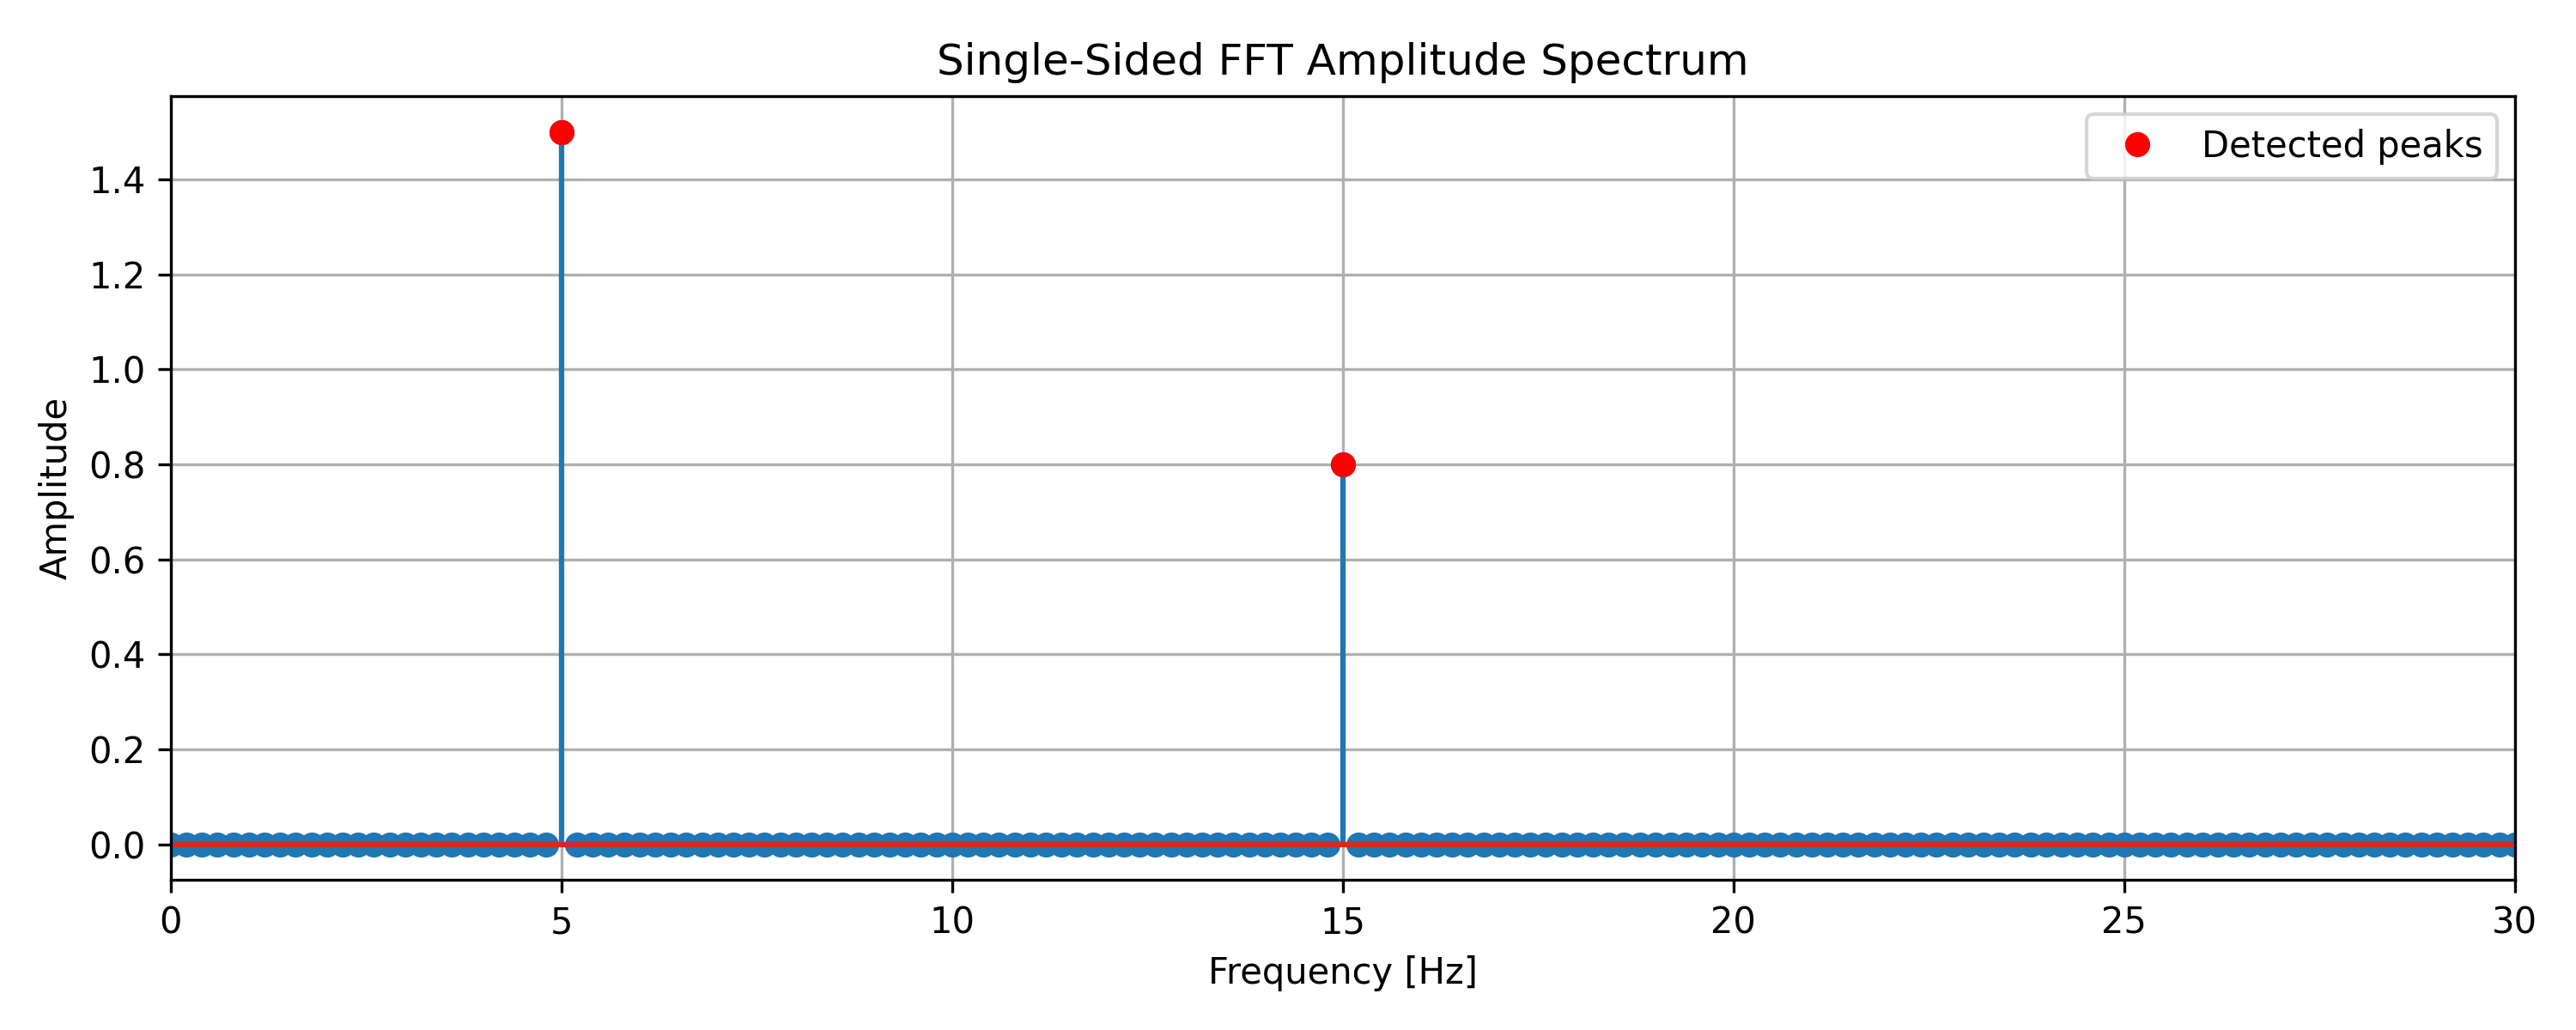
\includegraphics[width=\textwidth]{figures/exp01_amplitude_spectrum.png}
\caption{Single-sided FFT amplitude spectrum.}
\end{subfigure}
\caption{Synthetic vibration signal and corresponding FFT amplitude spectrum.}
\end{figure}

\subsubsection{Observations}

The frequency peaks appear at \(5\ \si{Hz}\) and \(15\ \si{Hz}\), matching the frequencies used to construct the signal. The amplitude scaling correctly recovers amplitudes close to \(1.5\) and \(0.8\).

\subsubsection{Discussion}

This experiment verifies the basic FFT workflow. For a clean synthetic signal with bin-centered frequencies, the FFT amplitude spectrum gives direct and accurate frequency identification.

% --------------------------------------------------
\subsection{Experiment 2: Phase Spectrum}

\subsubsection{Premise}

A synthetic signal is generated with known phase shifts. The objective is to compute and interpret the phase spectrum at the dominant frequency components.

\subsubsection{Signal Definition}

\begin{equation}
    x(t) =
    1.5 \sin(2\pi 5t + \pi/6)
    +
    0.8 \sin(2\pi 15t + \pi/3)
\end{equation}

\subsubsection{Parameters}

\begin{table}[H]
\centering
\caption{Parameters for phase spectrum experiment}
\begin{tabular}{ll}
\toprule
Parameter & Value \\
\midrule
Sampling frequency, \(f_s\) & \(100\ \si{Hz}\) \\
Duration, \(T\) & \(5\ \si{s}\) \\
Frequency component 1 & \(5\ \si{Hz}\) \\
Phase component 1 & \(\pi/6\) rad \\
Frequency component 2 & \(15\ \si{Hz}\) \\
Phase component 2 & \(\pi/3\) rad \\
\bottomrule
\end{tabular}
\end{table}

\subsubsection{Results}

The amplitude spectrum identifies the same dominant frequencies. The phase spectrum provides the phase angle associated with each frequency component.

\subsubsection{Generated Figure}

\begin{figure}[H]
\centering
\begin{subfigure}{0.48\textwidth}
\centering
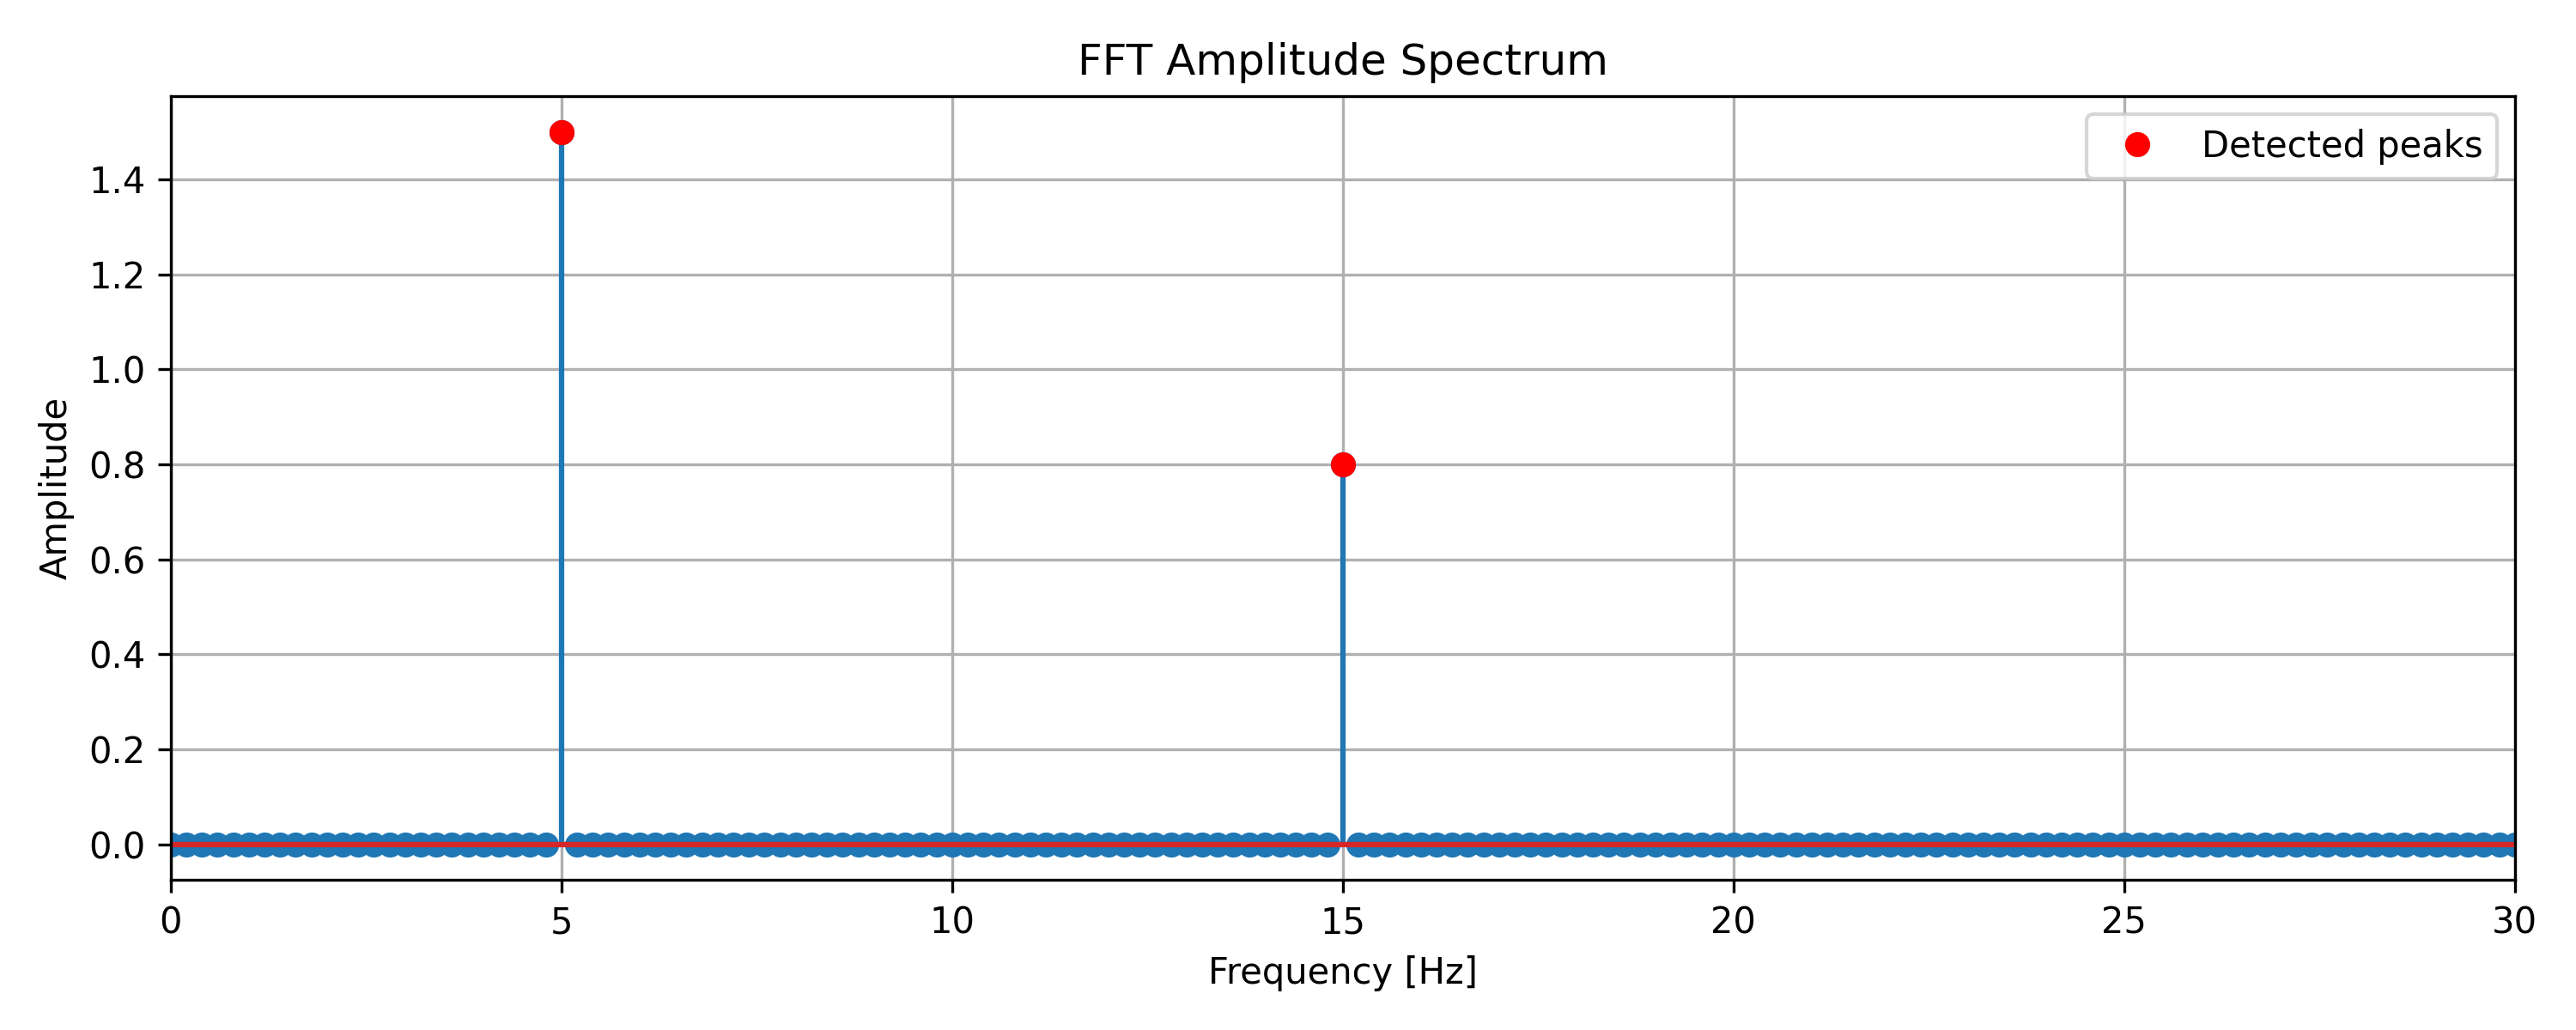
\includegraphics[width=\textwidth]{figures/exp02_amplitude_spectrum.png}
\caption{Amplitude spectrum.}
\end{subfigure}
\hfill
\begin{subfigure}{0.48\textwidth}
\centering
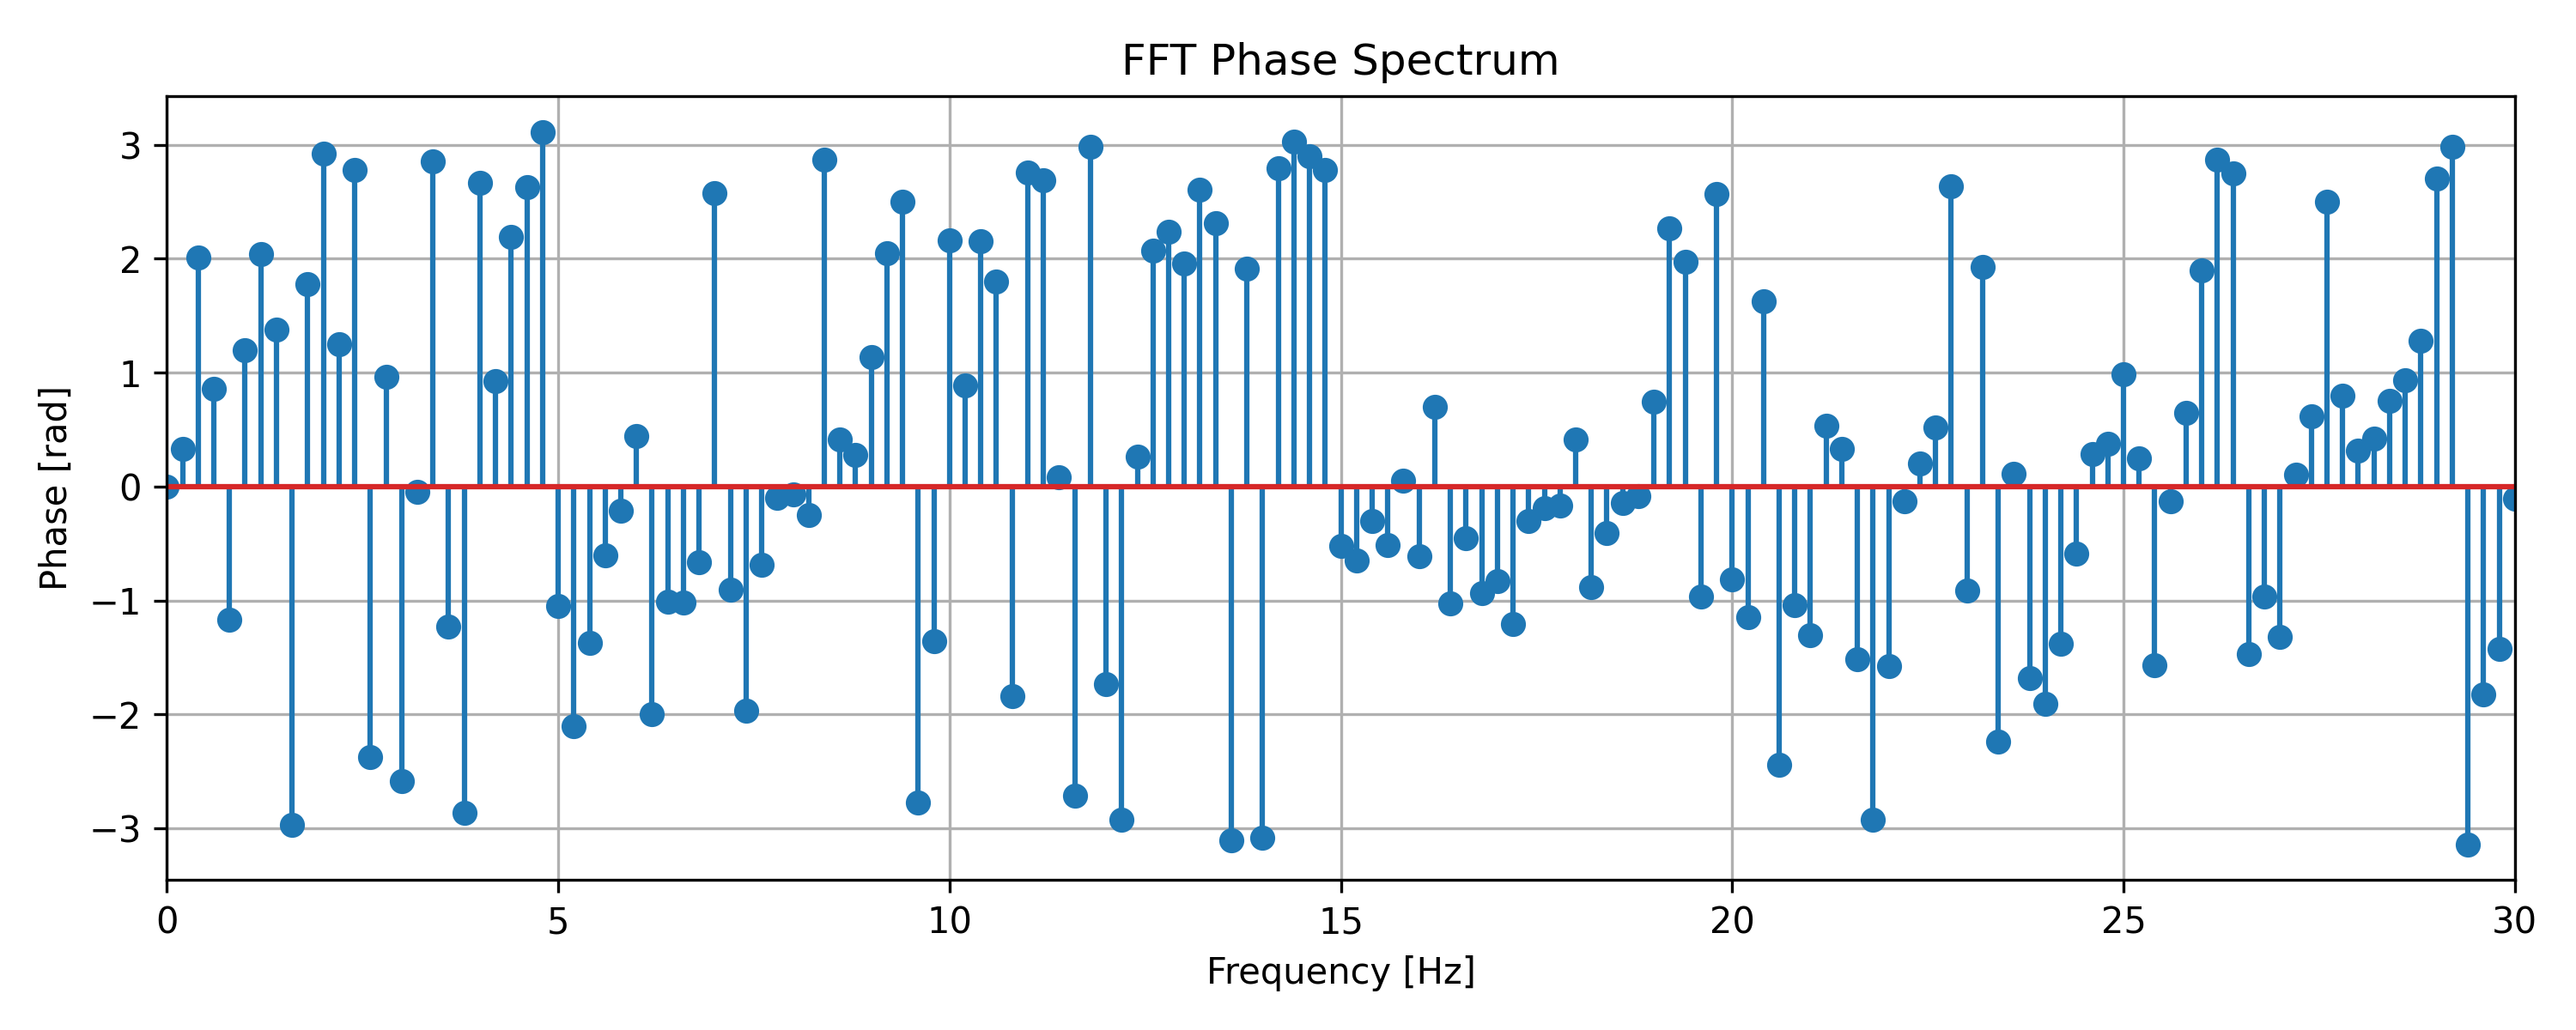
\includegraphics[width=\textwidth]{figures/exp02_phase_spectrum.png}
\caption{Phase spectrum.}
\end{subfigure}
\caption{FFT amplitude and phase spectra for a signal with phase-shifted components.}
\end{figure}

\subsubsection{Observations}

Changing the phase of the input signal changes the phase values in the FFT output. The amplitude peaks remain at the same frequencies because phase shift does not change the frequency content.

\subsubsection{Discussion}

Phase information is especially important when comparing multiple sensors. Two sensors may measure vibration at the same frequency, but the relative phase difference can indicate whether parts of the structure are moving in phase, out of phase, or with a time delay.

% --------------------------------------------------
\subsection{Experiment 3: Power Spectral Density Using Welch's Method}

\subsubsection{Premise}

A noisy vibration signal is analyzed using Welch's PSD estimate. The objective is to show that PSD analysis provides a smoother and more stable representation of frequency content in the presence of noise.

\subsubsection{Signal Definition}

\begin{equation}
    x(t) =
    1.5 \sin(2\pi 5t)
    +
    0.8 \sin(2\pi 15t)
    +
    \eta(t)
\end{equation}

where \(\eta(t)\) represents random noise.

\subsubsection{Parameters}

\begin{table}[H]
\centering
\caption{Parameters for Welch PSD experiment}
\begin{tabular}{ll}
\toprule
Parameter & Value \\
\midrule
Sampling frequency, \(f_s\) & \(100\ \si{Hz}\) \\
Duration, \(T\) & \(20\ \si{s}\) \\
Welch segment length, \(L\) & \(512\) samples \\
Window & Hann \\
Noise amplitude scale & \(0.5\) \\
Frequency component 1 & \(5\ \si{Hz}\) \\
Frequency component 2 & \(15\ \si{Hz}\) \\
\bottomrule
\end{tabular}
\end{table}

\subsubsection{Results}

The PSD is expected to show dominant energy concentration near:

\begin{equation}
    f = 5\ \si{Hz}
    \qquad \text{and} \qquad
    f = 15\ \si{Hz}
\end{equation}

\subsubsection{Generated Figure}

\begin{figure}[H]
\centering
\begin{subfigure}{0.48\textwidth}
\centering
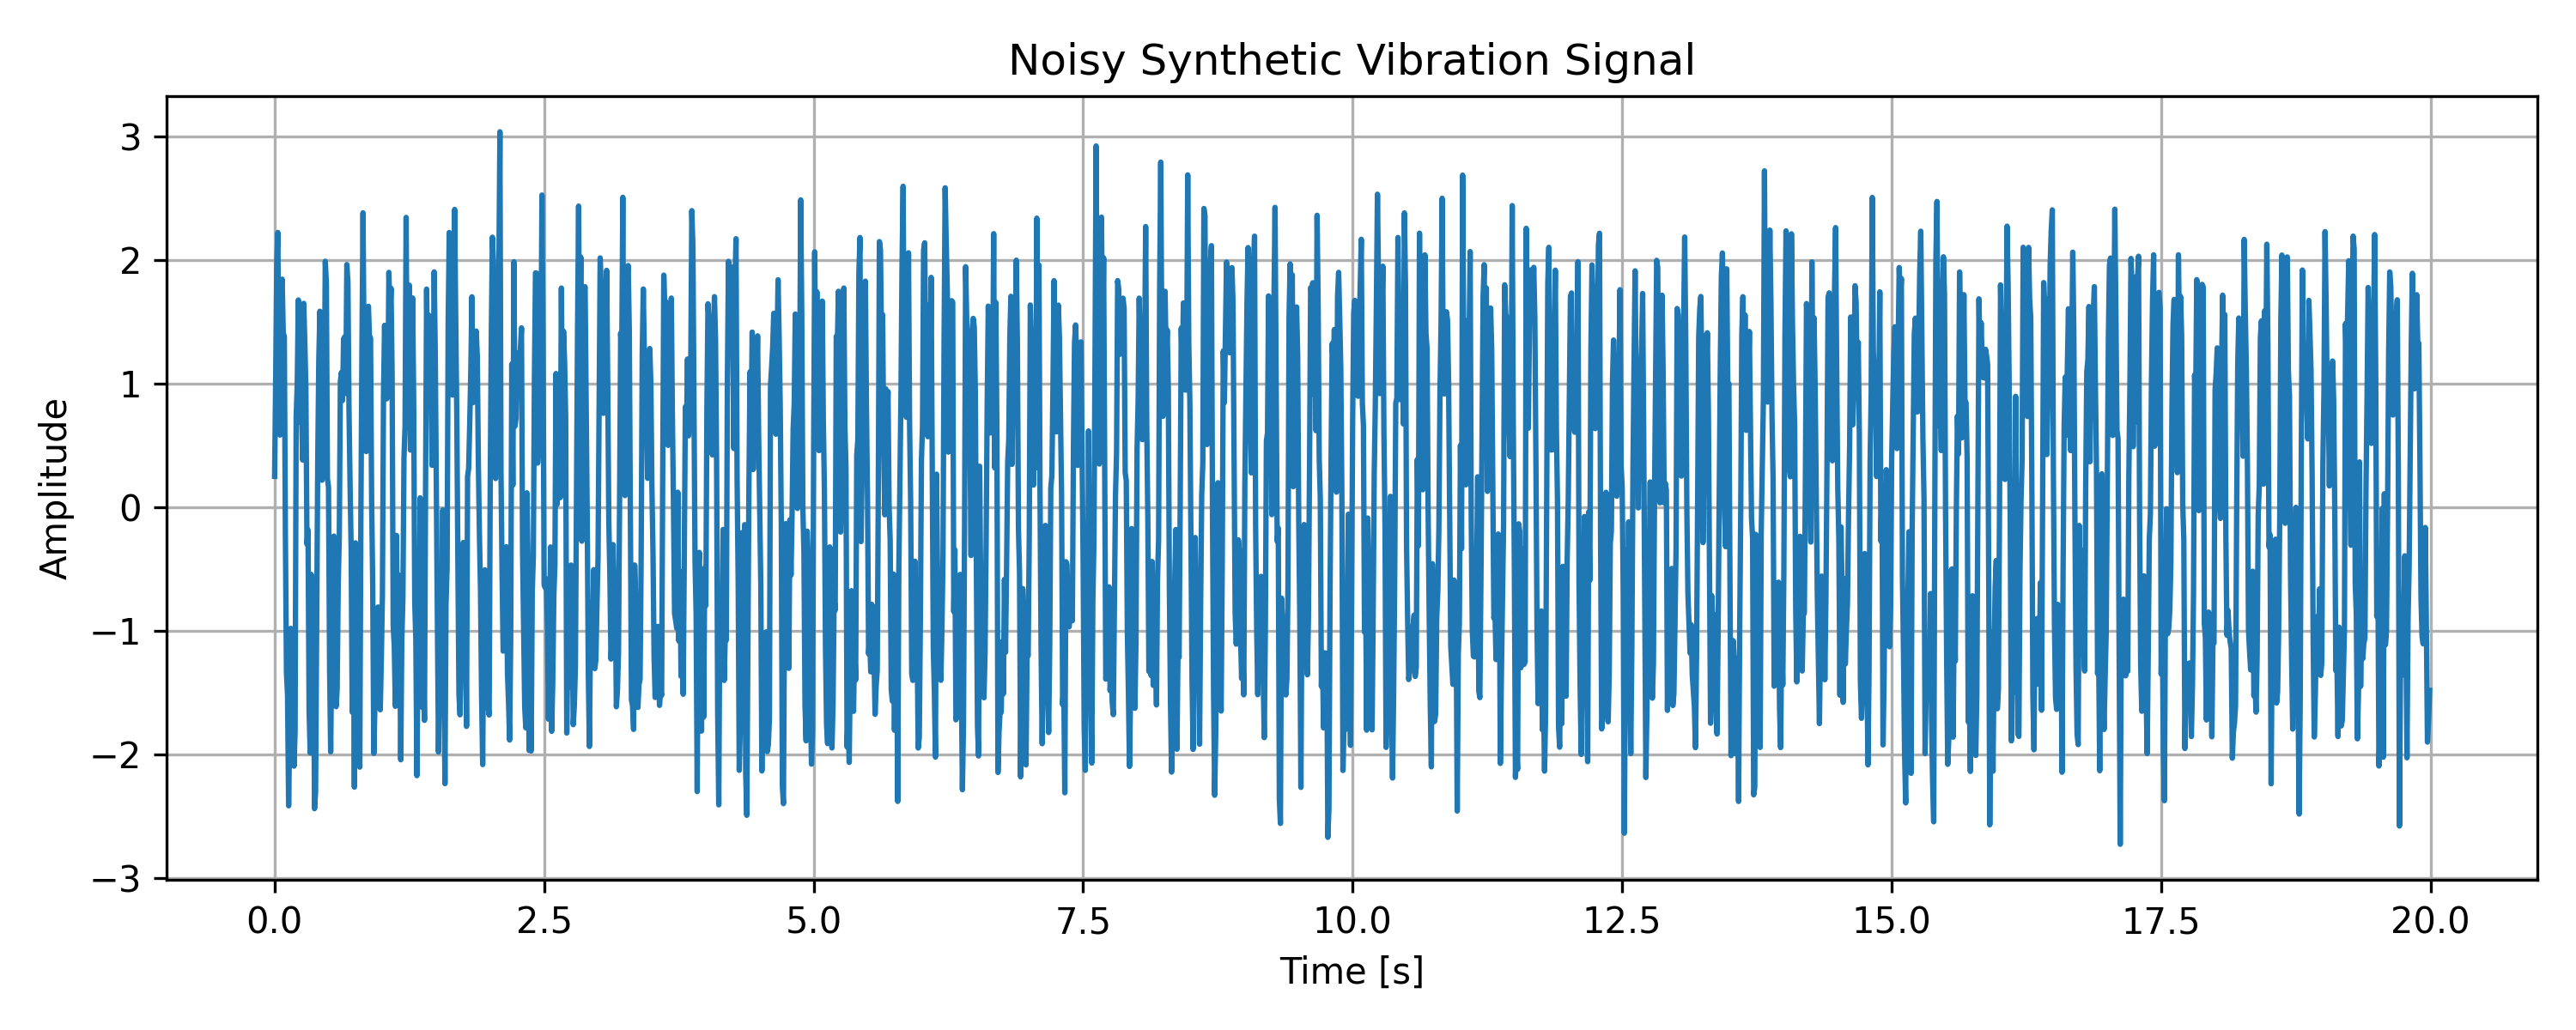
\includegraphics[width=\textwidth]{figures/exp03_noisy_time_signal.png}
\caption{Noisy time-domain signal.}
\end{subfigure}
\hfill
\begin{subfigure}{0.48\textwidth}
\centering
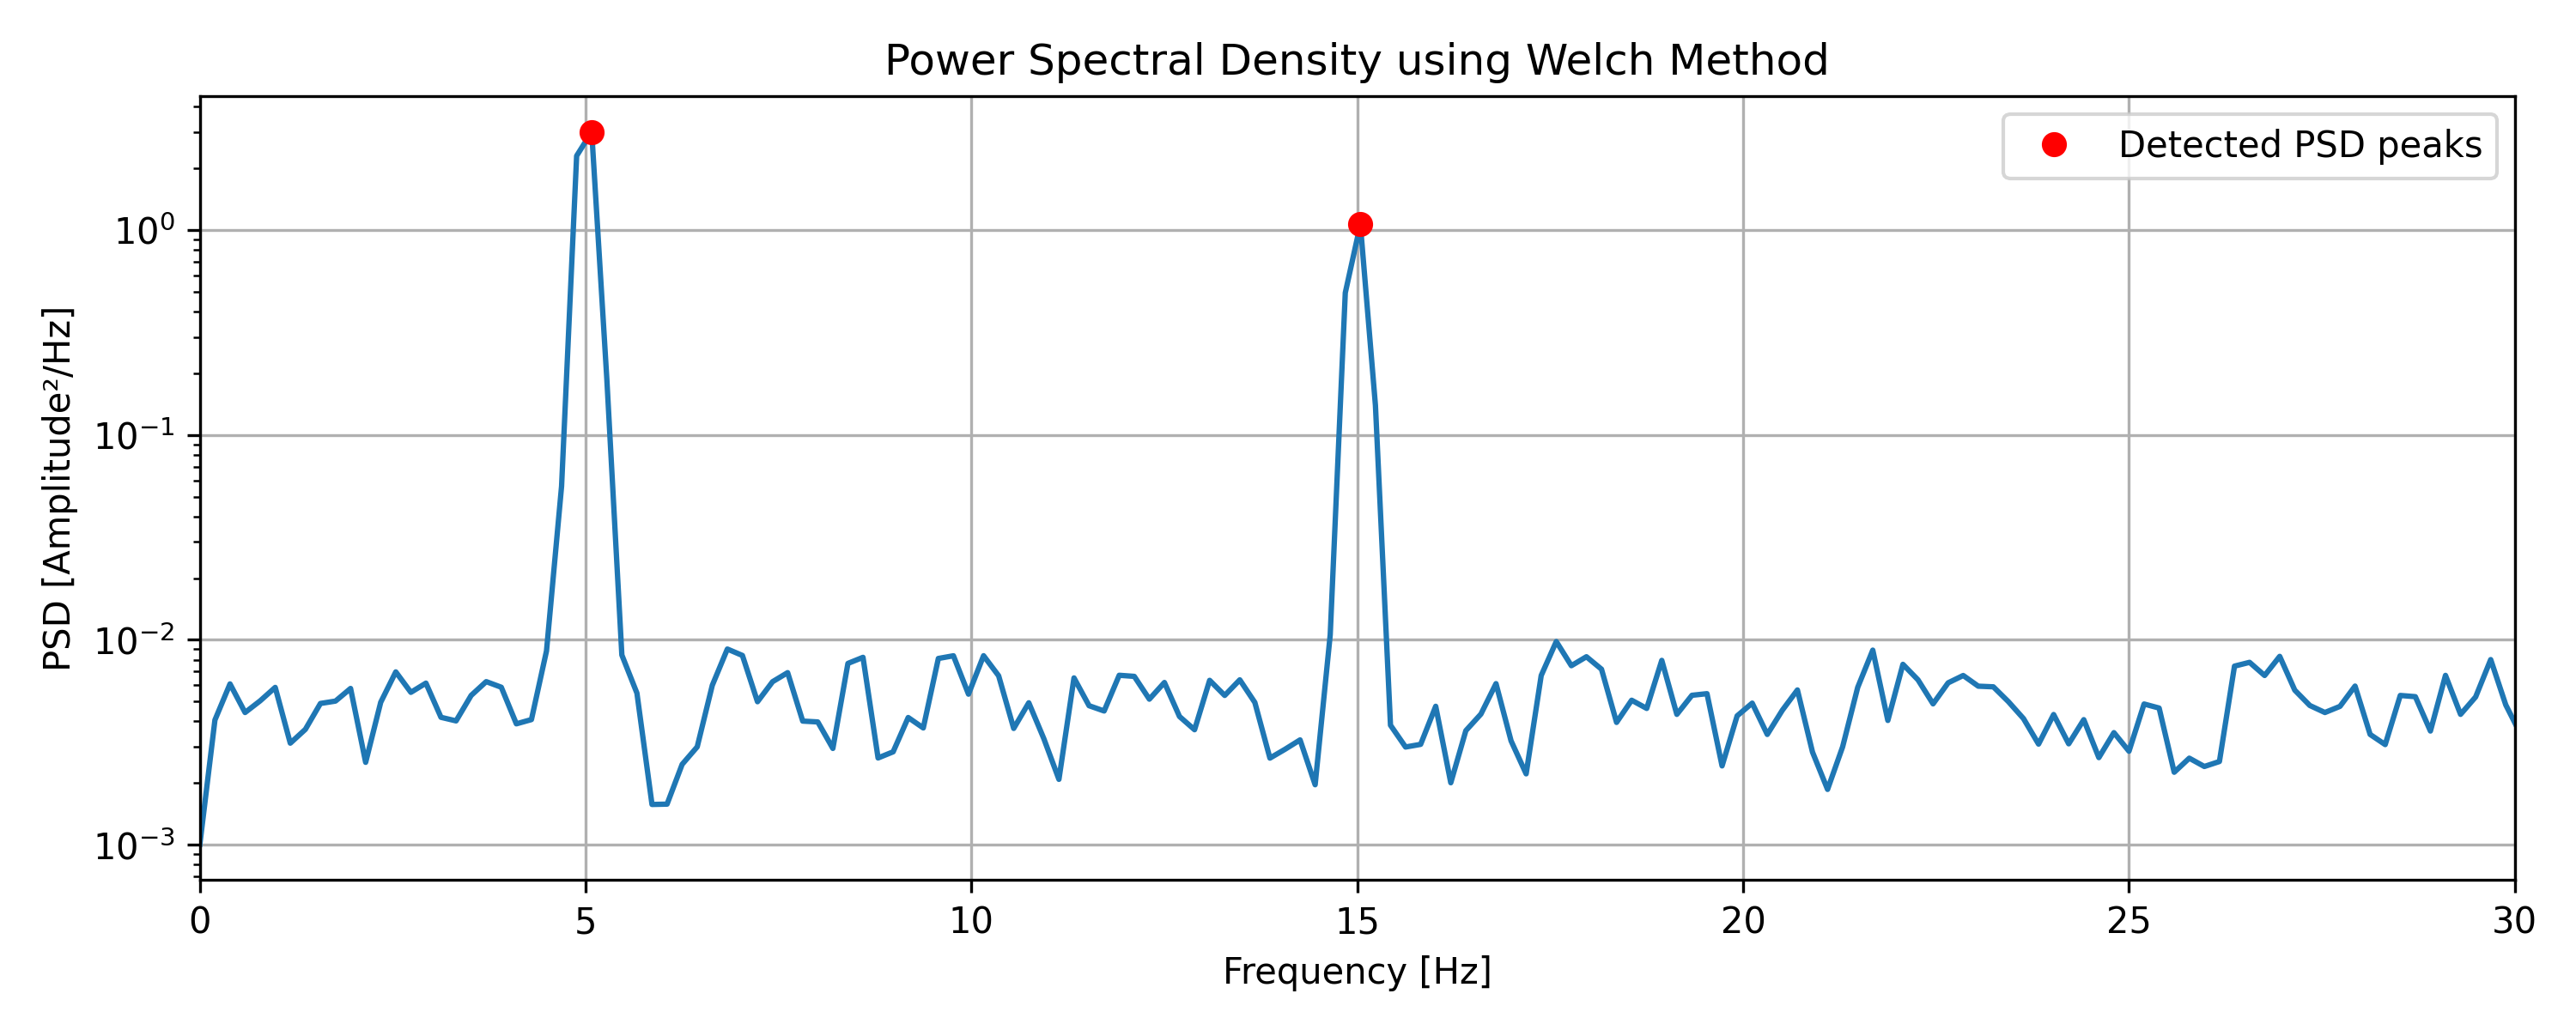
\includegraphics[width=\textwidth]{figures/exp03_welch_psd.png}
\caption{Welch PSD estimate.}
\end{subfigure}
\caption{Noisy vibration signal and PSD estimate using Welch's method.}
\end{figure}

\subsubsection{Observations}

Despite the presence of random noise, the PSD still shows clear peaks near the dominant frequency components. The PSD curve is smoother than a raw single FFT spectrum because Welch's method averages multiple segment spectra.

\subsubsection{Discussion}

Welch's method is useful for SHM because measured structural vibration data is often noisy and generated by ambient sources such as wind, traffic, machinery, and human activity. Averaging improves the stability of spectral estimates.

% --------------------------------------------------
\subsection{Experiment 4: Zero-Padding}

\subsubsection{Premise}

A sinusoidal signal with a non-bin-centered frequency is analyzed with and without zero-padding. The objective is to show that zero-padding creates a denser frequency grid but does not improve true physical frequency resolution.

\subsubsection{Signal Definition}

\begin{equation}
    x(t) =
    \sin(2\pi 5.3t)
\end{equation}

\subsubsection{Parameters}

\begin{table}[H]
\centering
\caption{Parameters for zero-padding experiment}
\begin{tabular}{ll}
\toprule
Parameter & Value \\
\midrule
Sampling frequency, \(f_s\) & \(100\ \si{Hz}\) \\
Duration, \(T\) & \(2\ \si{s}\) \\
Original number of samples, \(N\) & \(200\) \\
Original frequency spacing, \(\Delta f\) & \(0.5\ \si{Hz}\) \\
Zero-padded FFT length, \(N_{\text{pad}}\) & \(2048\) \\
Zero-padded spacing, \(\Delta f_{\text{pad}}\) & \(0.049\ \si{Hz}\) approximately \\
Signal frequency & \(5.3\ \si{Hz}\) \\
\bottomrule
\end{tabular}
\end{table}

\subsubsection{Results}

Zero-padding produces a smoother frequency-domain curve and a denser set of plotted frequency points.

\subsubsection{Generated Figure}

\begin{figure}[H]
\centering
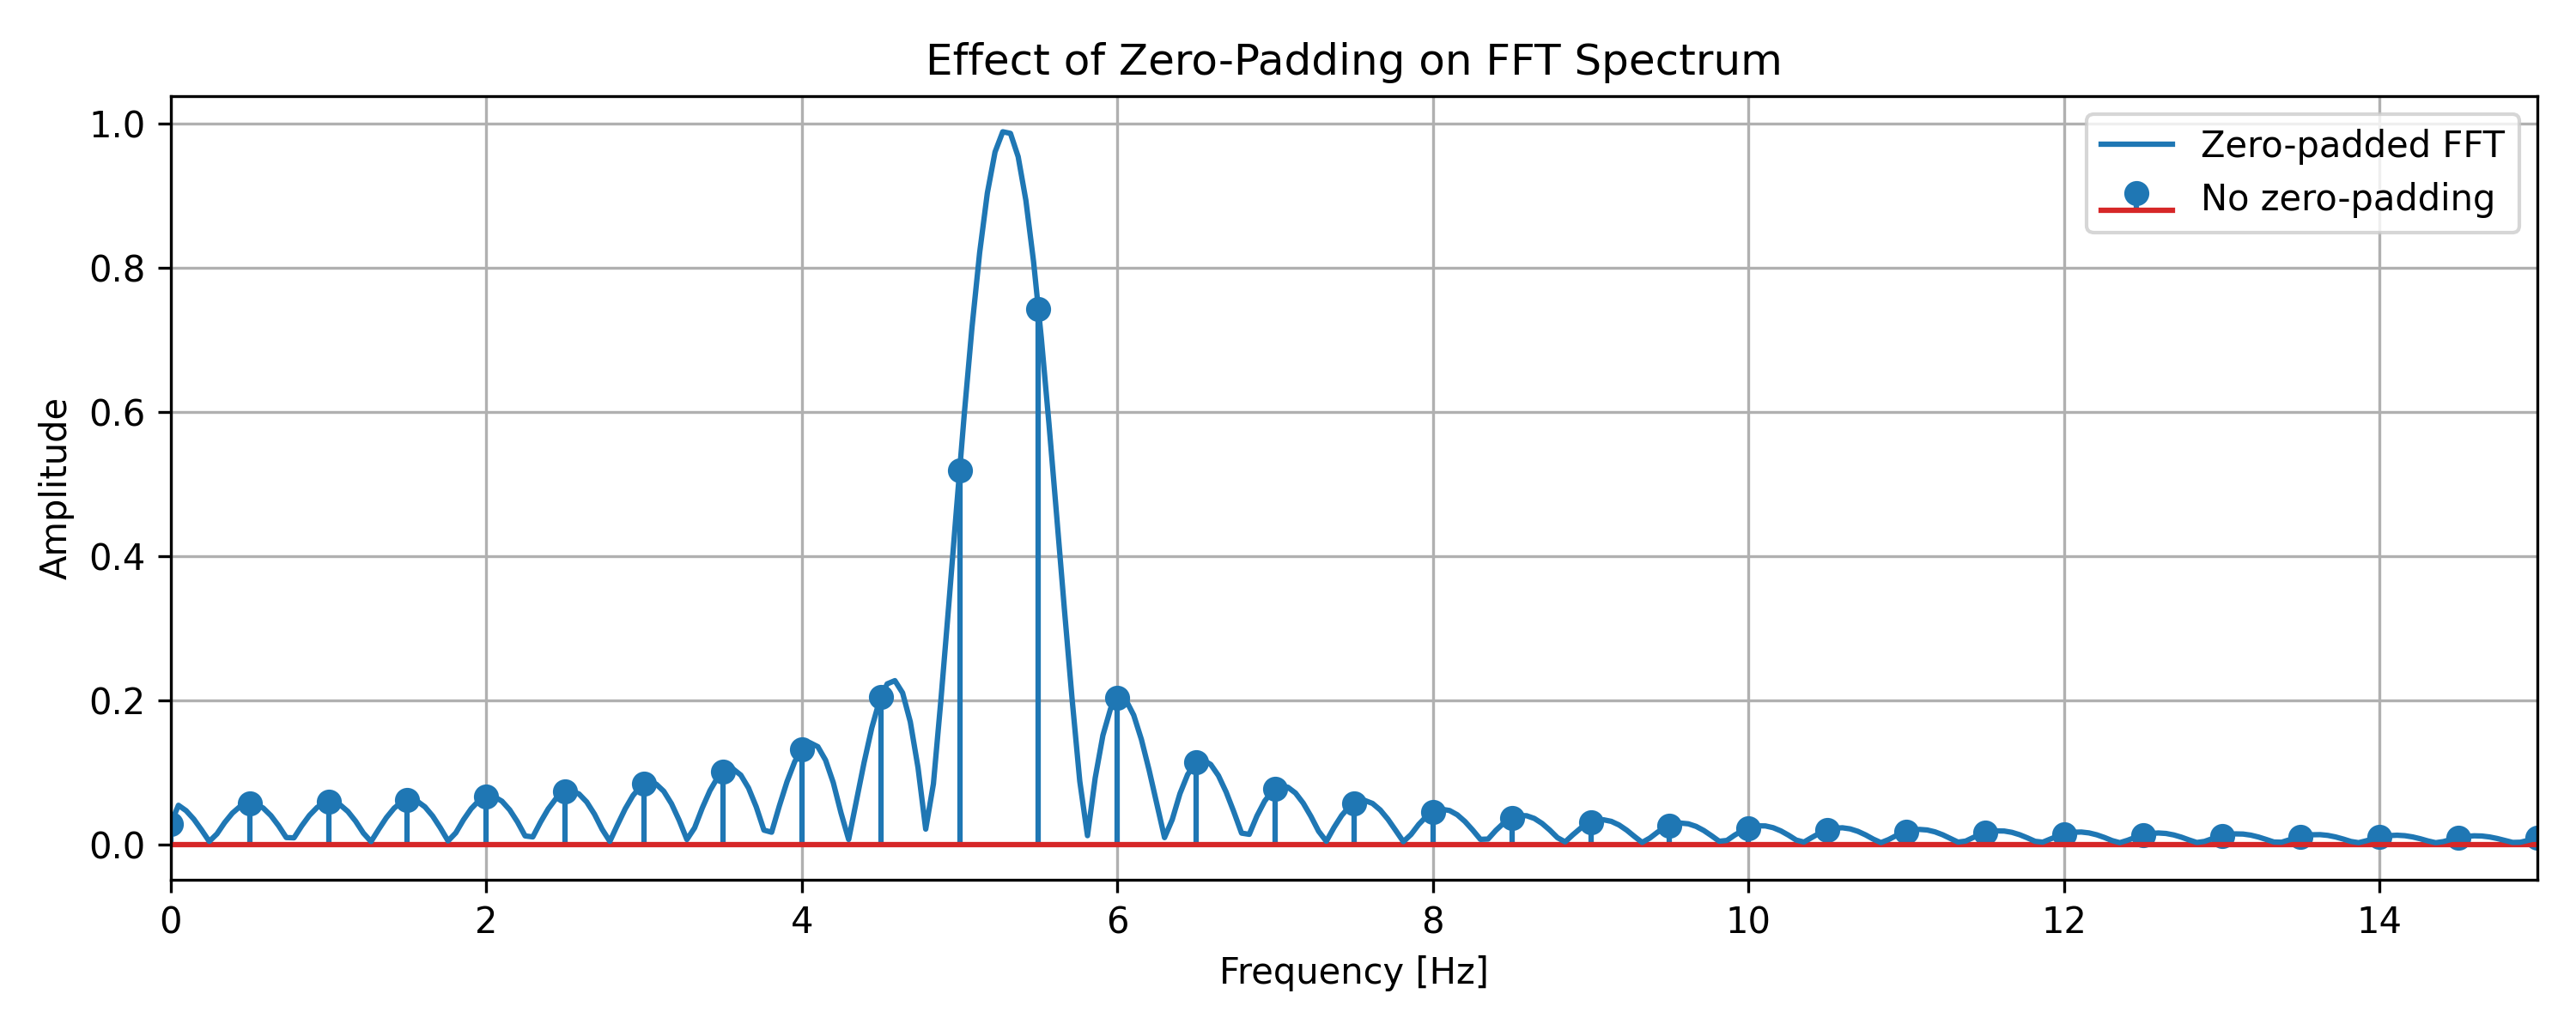
\includegraphics[width=0.85\textwidth]{figures/exp04_zero_padding.png}
\caption{Effect of zero-padding on FFT spectrum visualization.}
\end{figure}

\subsubsection{Observations}

The zero-padded FFT appears smoother and allows the peak region to be visually localized more clearly. However, no new measured vibration information is added.

\subsubsection{Discussion}

True frequency resolution depends on the actual duration of the measured signal. For better physical resolution, a longer measurement duration is required. Zero-padding is useful for visualization, but it should not be interpreted as an improvement in measurement quality.

% --------------------------------------------------
\subsection{Experiment 5: Harmonic Detection}

\subsubsection{Premise}

A signal containing harmonics of a fundamental frequency is generated. The objective is to automatically detect frequency peaks and classify them as harmonic components.

\subsubsection{Signal Definition}

\begin{equation}
    x(t) =
    1.0\sin(2\pi f_0t)
    +
    0.6\sin(2\pi 2f_0t)
    +
    0.3\sin(2\pi 3f_0t)
    +
    0.2\sin(2\pi 4f_0t)
\end{equation}

where:

\begin{equation}
    f_0 = 5\ \si{Hz}
\end{equation}

\subsubsection{Parameters}

\begin{table}[H]
\centering
\caption{Parameters for harmonic detection experiment}
\begin{tabular}{ll}
\toprule
Parameter & Value \\
\midrule
Sampling frequency, \(f_s\) & \(200\ \si{Hz}\) \\
Duration, \(T\) & \(5\ \si{s}\) \\
Fundamental frequency, \(f_0\) & \(5\ \si{Hz}\) \\
Harmonics included & \(f_0,\ 2f_0,\ 3f_0,\ 4f_0\) \\
Harmonic tolerance & \(0.05\) \\
\bottomrule
\end{tabular}
\end{table}

\subsubsection{Results}

\begin{table}[H]
\centering
\caption{Expected harmonic components}
\begin{tabular}{lll}
\toprule
Harmonic Number & Frequency & Amplitude \\
\midrule
1 & \(5\ \si{Hz}\) & \(1.0\) \\
2 & \(10\ \si{Hz}\) & \(0.6\) \\
3 & \(15\ \si{Hz}\) & \(0.3\) \\
4 & \(20\ \si{Hz}\) & \(0.2\) \\
\bottomrule
\end{tabular}
\end{table}

\subsubsection{Generated Figure}

\begin{figure}[H]
\centering
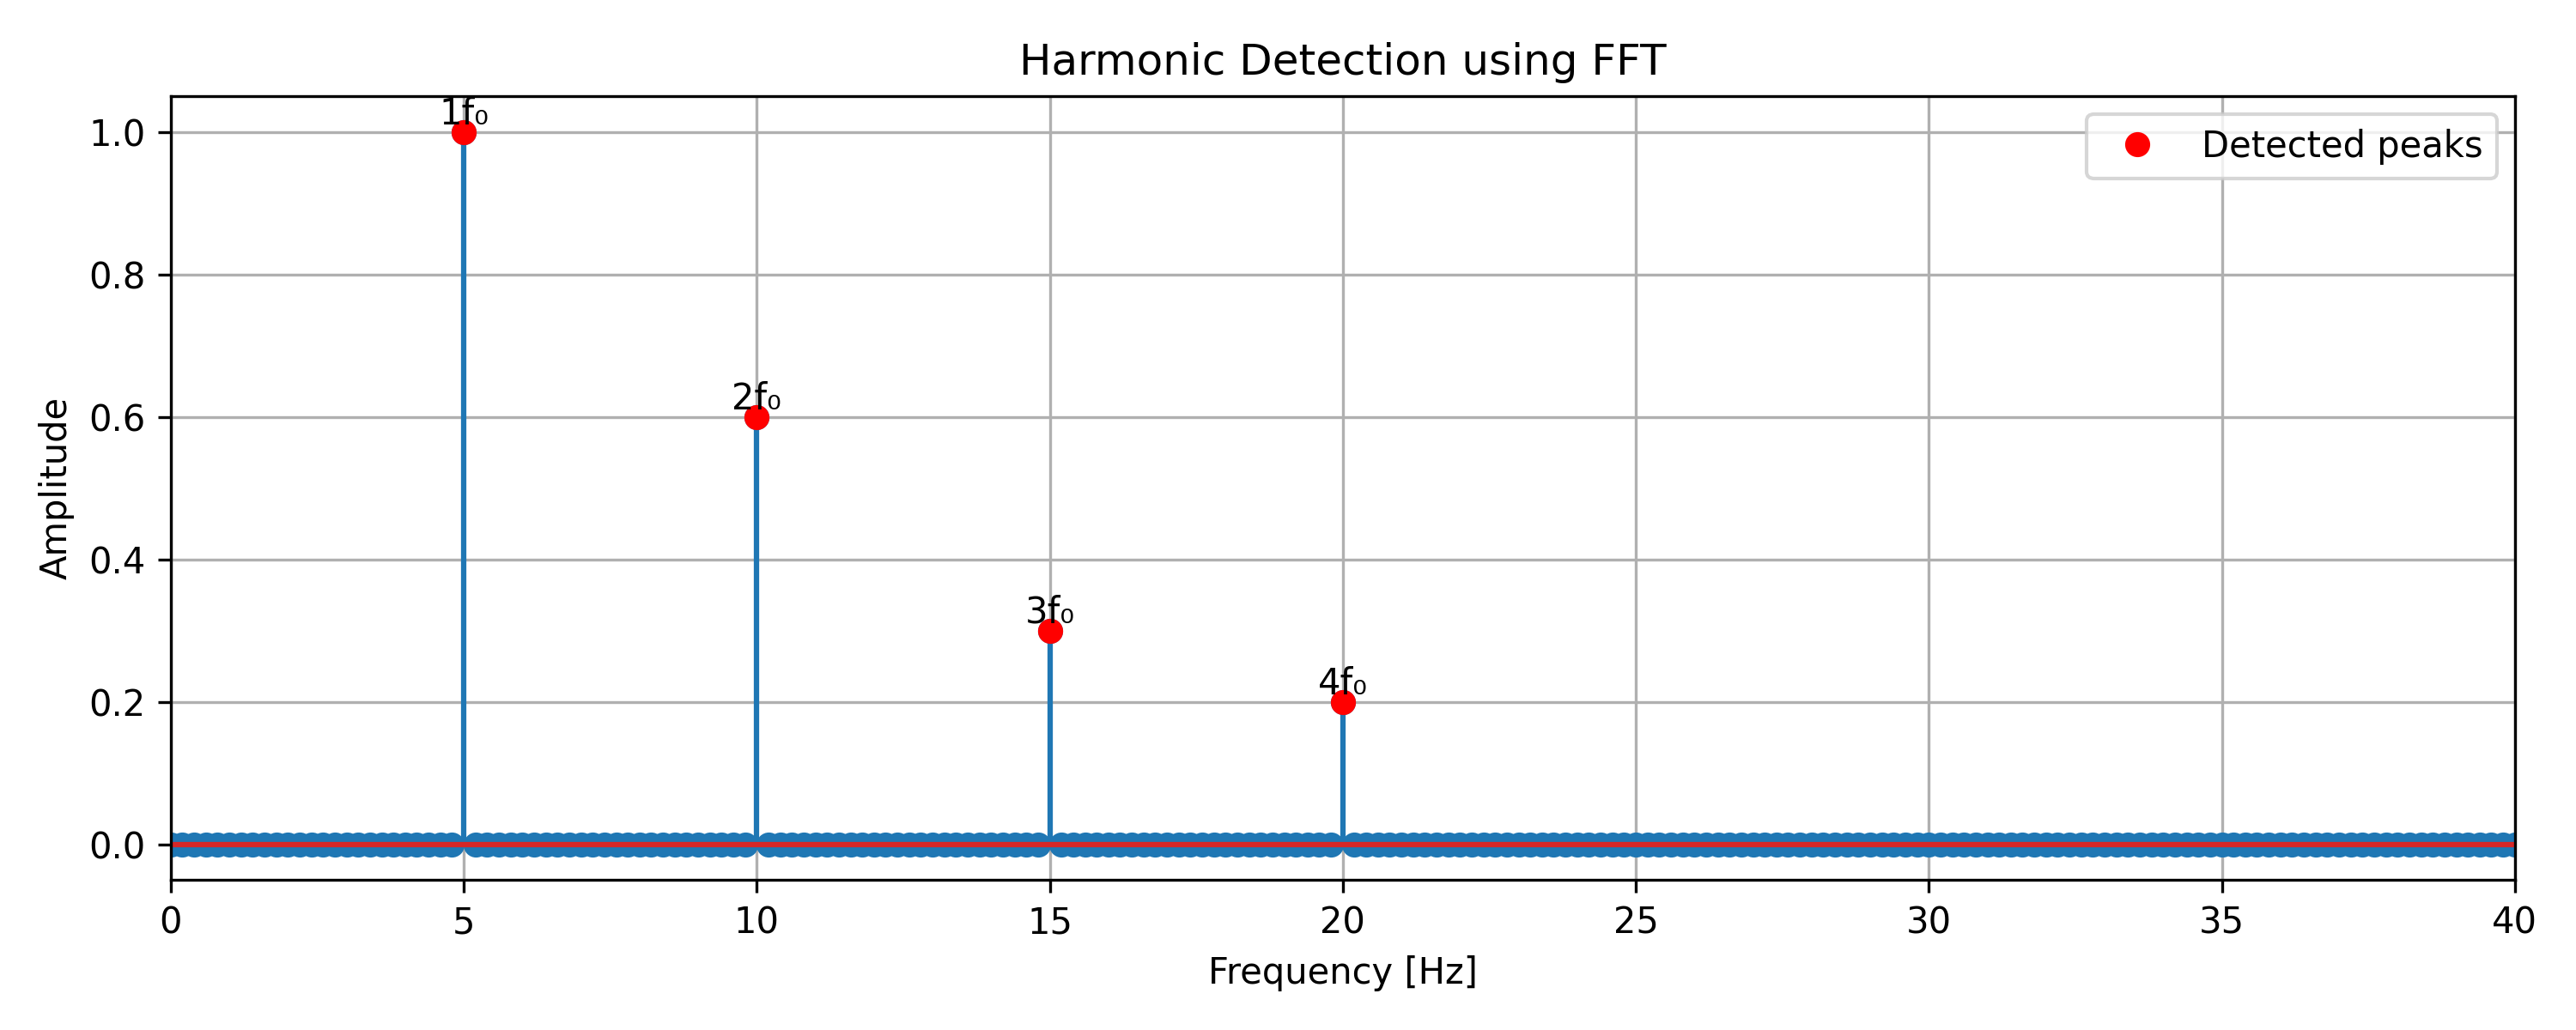
\includegraphics[width=0.85\textwidth]{figures/exp05_harmonic_detection.png}
\caption{Harmonic detection from FFT amplitude spectrum.}
\end{figure}

\subsubsection{Observations}

The algorithm identifies the fundamental frequency and detects peaks at integer multiples of this frequency.

\subsubsection{Discussion}

Harmonic detection is useful when analyzing periodic excitation sources. However, harmonics should not automatically be interpreted as structural natural frequencies. In SHM, it is important to distinguish between excitation frequencies and structural resonance frequencies.

% --------------------------------------------------
\subsection{Experiment 6: Spectral Leakage and Windowing}

\subsubsection{Premise}

A sinusoidal signal with a non-bin-centered frequency is analyzed with and without a Hann window. The objective is to demonstrate spectral leakage and the role of windowing.

\subsubsection{Signal Definition}

\begin{equation}
    x(t) =
    \sin(2\pi 5.3t)
\end{equation}

\subsubsection{Parameters}

\begin{table}[H]
\centering
\caption{Parameters for spectral leakage and windowing experiment}
\begin{tabular}{ll}
\toprule
Parameter & Value \\
\midrule
Sampling frequency, \(f_s\) & \(100\ \si{Hz}\) \\
Duration, \(T\) & \(2\ \si{s}\) \\
Number of samples, \(N\) & \(200\) \\
Frequency spacing, \(\Delta f\) & \(0.5\ \si{Hz}\) \\
Signal frequency & \(5.3\ \si{Hz}\) \\
Window type & Hann \\
\bottomrule
\end{tabular}
\end{table}

\subsubsection{Results}

The unwindowed FFT shows leakage into neighboring bins because the signal frequency does not fall exactly on an FFT bin. The Hann window reduces leakage away from the main peak but broadens the main lobe.

\subsubsection{Generated Figure}

\begin{figure}[H]
\centering
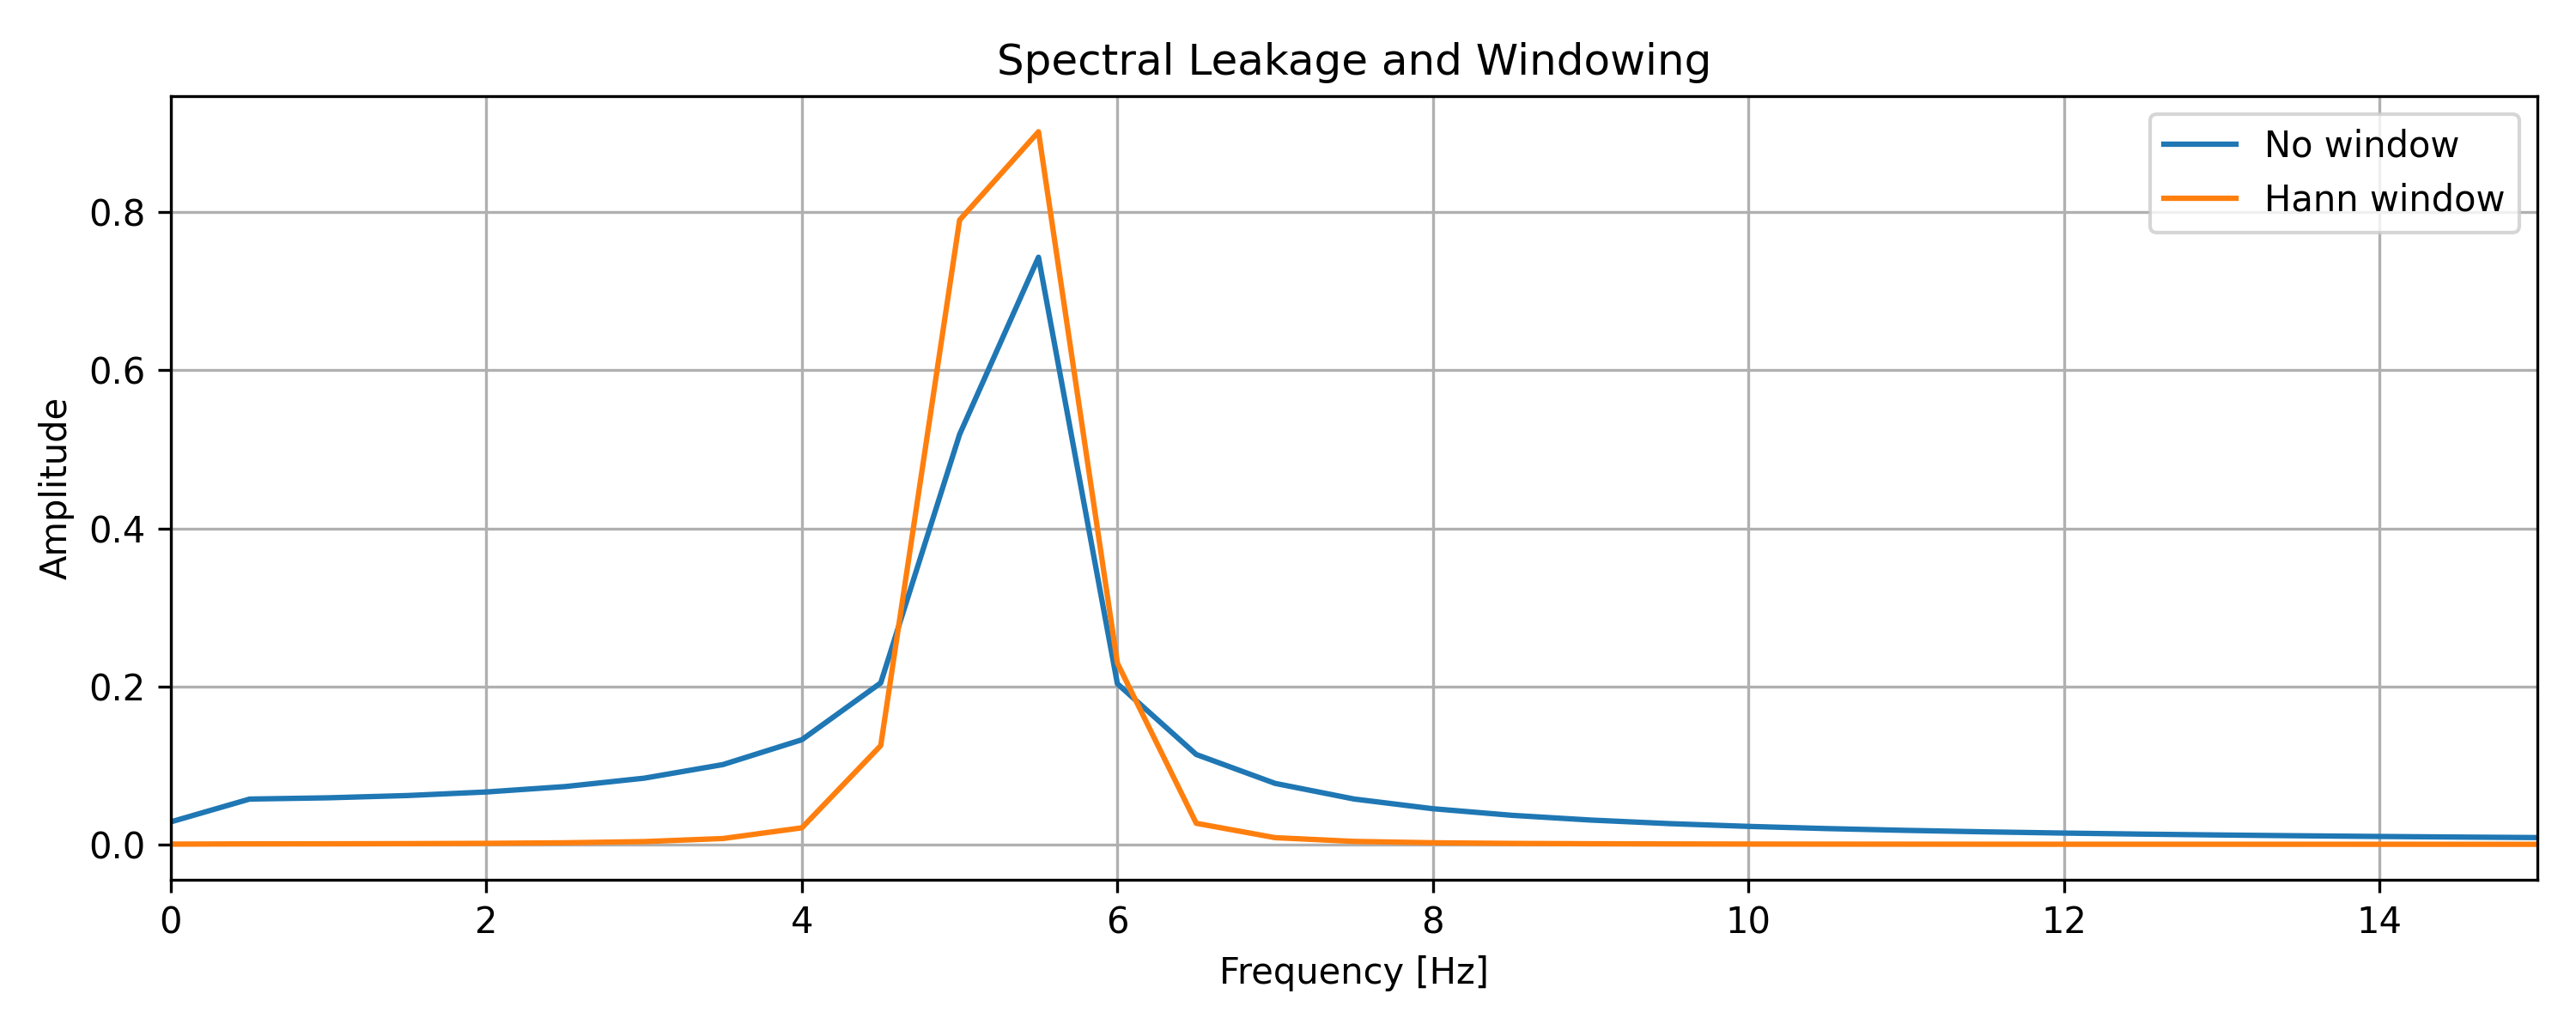
\includegraphics[width=0.85\textwidth]{figures/exp06_spectral_leakage_windowing.png}
\caption{Spectral leakage reduction using a Hann window.}
\end{figure}

\subsubsection{Observations}

Windowing changes the shape of the spectrum. It reduces leakage at frequencies far from the main peak but may make the main peak wider.

\subsubsection{Discussion}

In practical vibration measurements, the recorded time window rarely contains an exact integer number of cycles. Spectral leakage is therefore common. Windowing is a practical tool for improving frequency-domain interpretation.

% --------------------------------------------------
\section{Practical Example}
% --------------------------------------------------

Consider an accelerometer installed on a building floor. The sensor records acceleration response due to ambient vibration from wind, machinery, or traffic. The raw signal is measured as:

\begin{equation}
    a(t)
\end{equation}

After sampling, the discrete signal becomes:

\begin{equation}
    a[n]
\end{equation}

Using FFT-based frequency analysis, the dominant frequencies in the response can be extracted. If a clear peak appears near \(2.0\ \si{Hz}\), this may correspond to a dominant structural vibration mode or an excitation frequency.

If repeated monitoring shows that this peak shifts from:

\begin{equation}
    2.0\ \si{Hz}
    \quad \text{to} \quad
    1.8\ \si{Hz}
\end{equation}

then this may indicate a reduction in effective stiffness, assuming environmental and operational effects have been accounted for.

For noisy ambient data, Welch's PSD estimate is preferred because it gives a more stable estimate of the frequency content.

% --------------------------------------------------
\section{Summary}
% --------------------------------------------------

Stage 2 developed a practical FFT-based frequency analysis workflow. The completed tools include:

\begin{itemize}
    \item single-sided FFT amplitude spectrum,
    \item phase spectrum,
    \item automatic peak detection,
    \item Welch PSD estimation,
    \item zero-padding comparison,
    \item harmonic detection,
    \item spectral leakage and Hann windowing demonstration.
\end{itemize}

The main computational result is the ability to move from a time-domain vibration signal to interpretable frequency-domain features.

\begin{table}[H]
\centering
\caption{Summary of Stage 2 concepts}
\begin{tabular}{lll}
\toprule
Concept & Main Purpose & SHM Relevance \\
\midrule
FFT amplitude spectrum & Identify dominant frequencies & Natural frequency tracking \\
Phase spectrum & Measure phase shift & Multi-sensor comparison \\
PSD & Estimate power distribution & Noisy ambient vibration analysis \\
Zero-padding & Densify frequency grid & Spectrum visualization \\
Harmonic detection & Identify integer multiples & Excitation source characterization \\
Windowing & Reduce leakage & Cleaner spectral interpretation \\
\bottomrule
\end{tabular}
\end{table}

% --------------------------------------------------
\section{Engineering Notes}
% --------------------------------------------------

\begin{itemize}
    \item The FFT output must be scaled correctly before interpreting amplitudes.
    \item The frequency axis must be generated using the sampling frequency.
    \item The frequency resolution depends on total signal duration.
    \item Zero-padding does not improve true physical frequency resolution.
    \item PSD is more reliable than a raw FFT when analyzing noisy vibration data.
    \item Windowing reduces spectral leakage but changes the spectral shape.
    \item Harmonic frequencies are not automatically structural natural frequencies.
    \item Phase becomes important when comparing response between multiple sensors.
\end{itemize}

% --------------------------------------------------
\section{Conclusion}
% --------------------------------------------------

Stage 2 established the core frequency-domain analysis tools required for vibration-based structural monitoring. The FFT was used to transform time-domain signals into frequency-domain spectra, while amplitude scaling, phase extraction, PSD estimation, zero-padding, harmonic detection, and windowing were implemented as separate engineering experiments.

The stage provides a foundation for later work in modal identification, operational modal analysis, damage-sensitive feature extraction, and vibration-based structural health monitoring. The most important engineering outcome is the ability to correctly interpret spectral peaks and avoid common mistakes such as misreading zero-padding as improved frequency resolution or treating harmonic excitation frequencies as structural modes.

\end{document}
